\documentclass[12pt]{article}
\usepackage[paper=letterpaper,margin=2cm]{geometry}
\usepackage{amsmath}
\usepackage{amssymb}
\usepackage{amsfonts}
\usepackage{newtxtext, newtxmath}
\usepackage{enumitem}
\usepackage{titling}
\usepackage{multirow}
\usepackage{textcomp}
\usepackage{graphicx}
\usepackage{tikz}
\usepackage{listings}
\usepackage{xcolor}
\graphicspath{ {./images/} }

\definecolor{codegreen}{rgb}{0,0.6,0}
\definecolor{codegray}{rgb}{0.5,0.5,0.5}
\definecolor{codepurple}{rgb}{0.58,0,0.82}
\definecolor{backcolour}{rgb}{0.95,0.95,0.92}

\lstdefinestyle{mystyle}{
    backgroundcolor=\color{backcolour},   
    commentstyle=\color{codegreen},
    keywordstyle=\color{magenta},
    numberstyle=\tiny\color{codegray},
    stringstyle=\color{codepurple},
    basicstyle=\ttfamily\footnotesize,
    breakatwhitespace=false,         
    breaklines=true,                 
    captionpos=b,                    
    keepspaces=true,                 
    numbers=left,                    
    numbersep=5pt,                  
    showspaces=false,                
    showstringspaces=false,
    showtabs=false,                  
    tabsize=2
}

\lstset{style=mystyle}

\newdimen\nodeDist
\nodeDist=35mm
\usetikzlibrary{positioning}
\usepackage[colorlinks=true]{hyperref}

\setlength{\droptitle}{-6em}

\title{\large{Aprendizagem 2022}\vskip 0.2cm Homework I -- Group 58}
\date{}
\begin{document}
\maketitle
\center\large{\vskip -2.5cm\textbf{Part I}: Pen and paper}
\begin{enumerate}[leftmargin=\labelsep]
\item \leavevmode\vadjust{\vspace{-\baselineskip}}\newline\newline
\begin{tikzpicture}[
box/.style={draw,rectangle,minimum size=1.5cm,text width=1cm,align=center}]
\matrix (conmat) [row sep=0cm,column sep=0cm] {
\node (tpos) [box,
    label=left:\( \mathbf{P} \),
    label=above:\( \mathbf{P} \),
    ] {8};
&
\node (fneg) [box,
    label=above:\textbf{N}] {3};
\\
\node (fpos) [box,
    label=left:\( \mathbf{N} \)] {4};
&
\node (tneg) [box] {5};
\\
};
\node [left=.05cm of conmat,text width=1.5cm,align=right] {\textbf{actual \\ value}};
\node [above=.05cm of conmat] {\textbf{prediction outcome}};
\end{tikzpicture}

\item
Post-pruning of the given tree
under a maximum depth of 1:
\leavevmode\vadjust{\vspace{-\baselineskip}}\newline
\begin{center}
\begin{tikzpicture}[
    node/.style={%
      draw,
      rectangle,
    },
  ]

    \node [node] (A) {$y_1$};
    \path (A) ++(-135:\nodeDist) node [node] (B) {$\textbf{P} (5/7)$};
    \path (A) ++(-45:\nodeDist) node [node] (C) {$\textbf{N} (7/13)$};
        \draw (A) -- (B) node [left,pos=0.25] {A}(A);
    \draw (A) -- (C) node [right,pos=0.25] {B}(A);
\end{tikzpicture}
\hspace{1cm}
\begin{tikzpicture}[
box/.style={draw,rectangle,minimum size=1.5cm,text width=1cm,align=center}]
\matrix (conmat) [row sep=0cm,column sep=0cm] {
\node (tpos) [box,
    label=left:\( \mathbf{P} \),
    label=above:\( \mathbf{P} \),
    ] {5};
&
\node (fneg) [box,
    label=above:\textbf{N}] {6};
\\
\node (fpos) [box,
    label=left:\( \mathbf{N} \)] {2};
&
\node (tneg) [box] {7};
\\
};
\node [left=.05cm of conmat,text width=1.5cm,align=right] {\textbf{actual \\ value}};
\node [above=.05cm of conmat] {\textbf{prediction outcome}};
\end{tikzpicture}
\end{center}
\begin{math}
\newline
F1 = \frac{TP}{TP\ + \ \frac{1}{2}(FP \ + \ FN)}
\newline
\newline
F1 = \frac{5}{5 \ + \ \frac{1}{2}(2 \ + \ 6)} = \frac{5}{9}
\end{math}
\item
One reason why the left tree path was not further decomposed is because in the data set, 
whenever the variable $y_1$ had the value $A$, the class was always $P$, so there was no need to have more nodes.\newline
Another reason is due to reducing the tree 
complexity and increasing its efficiency and speed and, therefore, predictive power.

\item
\begin{math}
IG(class\ |\ y_1)=E(class) - E(class\ |\ y_1)
\newline
\newline
E(class) = - \sum_{x \in class} P(class = x)*\log_2[P(class = x)]
\newline
= -(\frac{11}{20}*\log_2\frac{11}{20} + \frac{9}{20}*\log_2\frac{9}{20})
\newline
\simeq 0.992774
\newline
\newline
E(class|y_1) = \sum_{x \in y_1} P(y_1 = x)*E(class|y_1=x)
\newline 
= \frac{7}{20}(-[\frac{5}{7}*\log_2\frac{5}{7}+ \frac{2}{7}*\log_2\frac{2}{7}]) + \frac{13}{20}(-[\frac{6}{13}*\log_2\frac{6}{13}+ \frac{7}{13}*\log_2\frac{7}{13}])
\newline
\simeq 0.949315
\newline
\newline
IG(class | y_1) = 0.992774 - 0.949315 \simeq 0.042459
\end{math}
\end{enumerate}

\center\large{\textbf{Part II}: Programming}

\begin{enumerate}[leftmargin=\labelsep,resume]
\item  \leavevmode\vadjust{\vspace{-\baselineskip}}\newline
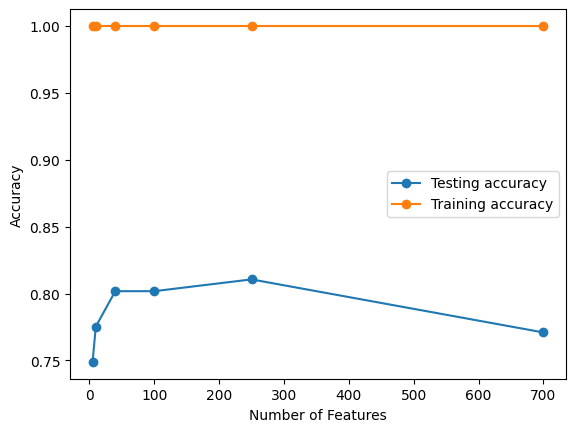
\includegraphics{plot}
\item
The training accuracy is persistently 1 because the data model is trained too well on 
our training data set, therefore, it predicts the correct values 100\% of the time on that 
data set.

\end{enumerate}
\newpage
\center\large{\textbf{Appendix}\vskip 0.3cm}

\begin{lstlisting}[language=Python]
from matplotlib import markers
import pandas as pd
from scipy.io.arff import loadarff
from sklearn.feature_selection import SelectKBest, mutual_info_classif
from sklearn.model_selection import train_test_split
from sklearn.tree import DecisionTreeClassifier
from sklearn import metrics
import matplotlib.pyplot as plt
import seaborn as sns
num_feat = [5, 10, 40, 100, 250, 700]
test_acc = []
train_acc = []

data = loadarff('pd_speech.arff')
df = pd.DataFrame(data[0])
df['class'] = df['class'].str.decode('utf-8')
X = df.drop('class', axis=1)
y = df['class']

for i in num_feat:
    X_new = SelectKBest(mutual_info_classif, k=i).fit_transform(X, y)
    X_train, X_test, y_train, y_test = train_test_split(X_new, y, train_size = 0.7, stratify = y,random_state = 1)
    classifier = DecisionTreeClassifier(random_state=1)
    classifier = classifier.fit(X_train, y_train)

    pred = classifier.predict(X_test)
    test_acc.append(metrics.accuracy_score(y_test, pred))
    train_acc.append(classifier.score(X_train, y_train))

fig, ax = plt.subplots()

ax.plot(num_feat, test_acc, label='Testing accuracy', marker='o')
ax.plot(num_feat, train_acc, label='Training accuracy', marker='o')
ax.set_xlabel("Number of Features")
ax.set_ylabel("Accuracy")
ax.legend()

plt.show()
\end{lstlisting}

\end{document}